\section{Tensorprodukte}

\begin{definition}[billineare Abbildung]
	Eine Abbildung $\xi:V\times W\to U$ ist \begriff[Abbildung!]{bilinear}, wenn für jedes $v\in V$ die Abbildung 
	\begin{align}
		\begin{cases}
		W\to U \\ w\mapsto \xi(v,w)
		\end{cases}\notag
	\end{align}
	und für jedes $w\in W$ die Abbildung
	\begin{align}
	\begin{cases}
	V\to U \\ v\mapsto \xi(v,w)
	\end{cases}\notag
	\end{align}
	linear sind.
	
	Wir definieren
	\begin{align}
		\Bil_K(V,W,U)=\{\xi\in\Abb(V\times W,U)\mid \xi\text{ bilinear}\}\notag
	\end{align}
\end{definition}

\begin{example}
	Seien $V=W=K[t]_{\le d}$, $U=K[t]_{\le 2d}$. Die Abbildung
	\begin{align}
	\xi:\begin{cases}
	V\times W\to U \\ (f.g)\mapsto fg
	\end{cases}\quad\text{ ist bilinear}\notag
	\end{align}
	Wir sehen, dass $\Image(\xi)$ im Allgemeinen kein Untervektorraum von $U$ ist. Ist zum Beispiel $K=\ratio$, $d=1$, so liegen $t^2=\xi(t,t)$ und $-2=\xi(-2,1)$ im $\Image(\xi)$ nicht jedoch $t^2-2$, denn wäre $t^2-2=fg$ mit $f,g\in\ratio[t]$ linear, so hätte $t^2-2$ eine Nullstelle in $\ratio$, aber $\sqrt{2}\notin\ratio$.
\end{example}

\begin{lemma}
	$\Bil_K(V,W,U)$ bildet einen Untervektorraum des $K$-Vektorraum $\Abb(V\times W,U)$.
\end{lemma}
\begin{proof}
	klar, zum Beispiel
	\begin{align}
		(\xi+\xi')(\lambda v,w)=\xi(\lambda v,w)+\xi'(\lambda v,w)=\lambda\xi(v,w)+\lambda\xi(v,w)= \lambda(\xi+\xi')(v,w)\notag
	\end{align}
\end{proof}

\begin{lemma}
	Ist $\xi\in\Bil_K(V,W,U)$ und $f\in\Hom_K(U,U')$ für einen $K$-Vektorraum, so ist 
	\begin{align}
		f\circ \xi\in\Bil_K(V,W,U')\notag
	\end{align}
\end{lemma}
\begin{proof}
	klar, zum Beispiel
	\begin{align}
		(f\circ\xi)(\lambda v,w)=f(\xi(\lambda v,w))=f(\lambda\xi(v,w))=\lambda\cdot(f\circ\xi)(v,w)\notag
	\end{align}
\end{proof}

\begin{lemma}
	\proplbl{3_6_5}
	Sei $(v_i)_{i\in I}$ eine Basis von $V$ und $(w_j)_{j\in J}$ eine Basis von $W$. Zu jeder Familie $(u_{ij})_{(i,j)\in I\times J}$ in $U$ gibt es genau ein $\xi\in\Bil_K(V,W,U)$ mit
	\begin{align}
		\xi(v_i,w_i)=u_{ij}\quad\forall i\in I, j\in J\notag
	\end{align}
\end{lemma}
\begin{proof}
	\begin{itemize}
		\item Eindeutigkeit: Ist $\xi$ bilinear, $v=\sum_{i\in I} \lambda_i v_i$, $w=\sum_{j\in J} \mu_j w_j$ so ist 
		\begin{align}
			\xi(v,w)&=\xi\left(\sum_{i\in I} \lambda_i v_i,\sum_{j\in J}\mu_j w_j\right) \notag \\
			&= \sum_{i\in I}\lambda_i\xi\left(v_i,\sum_{j\in J}\mu_j w_j\right)\notag \\
			&= \sum_{i,j}\lambda_i\mu_j u_{ij}
		\end{align}
		durch die Familie $(u_{ij})_{i,j}$ bestimmt.
		\item Existenz: Wird $\xi$ durch (1) definiert, so ist $\xi$ bilinear: Für festes $w=\sum_{j\in J}\mu_j w_j$ ist
		\begin{align}
			\begin{cases}
			V&\to U \\ v=\sum\limits_{i\in I}\lambda_i v_i&\mapsto \xi(v,w)=\sum\limits_{i\in I}\lambda_i\left(\sum\limits_{j\in J}\mu_j u_{ij}\right)
			\end{cases}\notag
		\end{align}
		linear (LAAG1 III.5.1), analog für festes $v$. %TODO: Verlinkung
	\end{itemize}
\end{proof}

\begin{definition}[Tensorprodukt]
	Ein \begriff{Tensorprodukt} von $V$ und $W$ ist ein Paar $(T,\tau)$ bestehend aus einem $K$-Vektorraum $T$ und einer bilinearen Abbildung $\tau\in\Bil_K(V,W,T)$ welche die folgende \begriff{universelle Eigenschaft} erfüllt: \\
	\textit{Ist $U$ ein weiterer $K$-Vektorraum und $\xi\in\Bil_K(V,W,U)$ so gibt es genau ein $\xi_\otimes\in\Hom_K(T,U)$ mit $\xi=\xi_\otimes\circ\tau$.}
	\begin{center}
		\begin{tikzpicture}
		\matrix (m) [matrix of math nodes,row sep=3em,column sep=4em,minimum width=2em]
		{V\times W & T \\ \; & U \\};
		\path[-stealth]
		(m-1-1) edge node [below] {$\xi$} (m-2-2)
		edge node [above] {$\tau$} (m-1-2)
		(m-1-2) edge [dashed] node [right] {$\xi_\otimes$} (m-2-2);
		\end{tikzpicture}
	\end{center}
\end{definition}

\begin{*anmerkung}
	Sind $V$ und $W$ zwei Vektorräume und $K$ ein gemeinsamer Körper, so kann man das Tensorprodukt $V\otimes W$, was auch ein Vektorraum ist, wie folgt konstruieren: Wenn $B=(b_1,...,b_n)$ eine Basis von $V$ und $C=(c_1,...,c_m)$ eine Basis von $W$ ist, dass ist $V\otimes W$ ein Vektorraum, genannt \textit{Tensorproduktraum}, in dem es eine Basis gibt, die auf eindeutige Weise mit den geordneten Paaren des kartesischen Produkts
	\begin{align}
		B\times C=\{(b_i,c_j)\}\notag
	\end{align}
	der Basen der Ausgangsräume identifiziert werden kann. Die Dimension von $V\otimes W$ ist dann das Produkt der Dimensionen von $V$ und $W$. Ein Element der Basis von $V\otimes W$, das dem Paar $(b_i,c_j)$ entspricht, wird als $b_i\otimes c_j$ notiert, das $\otimes$ hat also keine tiefere Bedeutung. Ein Element des Tensorproduktes $V\otimes W$ hat dann die Gestalt:
	\begin{align}
		\sum_{i,j} \lambda_{ij}\cdot (b_i\otimes c_j)\notag
	\end{align}
	mit $\lambda_{ij}\in K$.
\end{*anmerkung}

\begin{lemma}
	\proplbl{3_6_7}
	Sind $(T,\tau)$ und $(T',\tau')$ Tensorprodukte von $V$ und $W$, so gibt es einen eindeutig bestimmten Isomorphismus $\Theta:T\to T'$ mit $\tau'=\Theta\circ\tau$.
	\begin{center}
		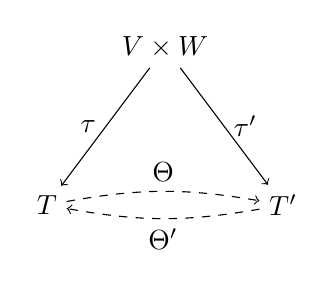
\begin{tikzpicture}
		\node (V) at (1.5,0) {$V\times W$};
		\node (T) at (0,-2) {$T$};
		\node (S) at (3,-2) {$T'$};
		\draw[->, left] (V) to node {$\tau$} (T);
		\draw[->, right] (V)  to node {$\tau'$} (S);
		\draw[->, above, dashed] (T)  to [bend left=10] node {$\Theta$} (S);
		\draw[->, below, dashed] (S)  to [bend left=10] node {$\Theta'$} (T);
		\end{tikzpicture}
	\end{center}
\end{lemma}
\begin{proof}
	Da $(T,\tau)$ die universelle Eigenschaft erfüllt, gibt es ein eindeutig bestimmtes $\Theta=(\tau')_\otimes\in\Hom_K(T,T')$ mit $\tau'=\Theta\circ\tau$. Analog gibt es $\Theta'\in\Hom_K(T',T)$ mit $\tau=\Theta'\circ\tau'$. Es folgt, dass $\tau=\Theta'\circ\tau'= \Theta'\circ\Theta\circ\tau$. Da auch $\tau=\id_T\circ\tau$ liefert die Eindeutigkeitsaussage in der universellen Eigenschaft von $(T,\tau)$, für $U=T$, $\xi=\tau$, dass $\Theta\circ\Theta'=\id_T$. Analog sieht man, dass $\Theta\circ\Theta'=\id_{T'}$. Somit ist $\Theta$ ein Isomorphismus.
\end{proof}

\begin{definition}[Vektorraum mit Basis $X$]
	\proplbl{3_6_8}
	Sei $X$ eine Menge. Der $K$-\begriff{Vektorraum mit Basis $X$} ist der Untervektorraum $V=\Span_K((\delta_x)_{x\in X})$ des $K$-Vektorraum $\Abb(X,K)$ mit $\delta_x(y)=\delta_{x,y}=\begin{cases}1&x=y\\0&x\neq y\end{cases}$
\end{definition}

\begin{lemma}
	Sei $X$ eine Menge und $V$ der $K$-Vektorraum mit Basis $X$. Dann ist $V$ ein $K$-Vektorraum und $(\delta_x)_{x\in X}$ ist eine Basis von $V$.
\end{lemma}
\begin{proof}
	Zu zeigen ist nur, dass $(\delta_x)_{x\in X}$ linear unabhängig ist. Ist $f=\sum_{x\in X}\lambda_x \delta_x$, $\lambda_x\in K$, fast alle gleich 0, und $f=0$, so ist $\lambda_x=f(x)=0$ für jedes $x\in X$. 
\end{proof}

\begin{lemma}
	\proplbl{3_6_10}
	Sei $(v_i)_{i\in I}$ eine Basis von $V$ und $(w_j)_{j\in J}$ eine Basis von $W$. Sei $T$ der $K$-Vektorraum mit der Basis $I\times J$ (im Sinne von \propref{3_6_8}) und $\tau:V\times W\to T$ die bilineare Abbildung gegeben durch $(v_i,w_j)\mapsto \delta_{i,j}$, vergleiche \propref{3_6_5}. Dann ist $(T,\tau)$ ein Tensorprodukt von $V$ und $W$.
\end{lemma}
\begin{proof}
	Wir schreiben $v_i\otimes w_j$ für $\delta_{i,j}$. Sei $U$ ein weiterer $K$-Vektorraum und $\xi\in\Bil_K(V,W,U)$. Da $(v_i\otimes w_j)_{(ij)\in I\times J}$ eine Basis von $T$ ist, gibt es genau ein $\xi_\otimes\in\Hom_K(T,U)$ mit $\xi_\otimes(v_i\otimes w_j)=\xi(v_i,w_j)$ für alle $i,j$, also mit $\xi_\otimes\circ\tau=\xi$ nach \propref{3_6_5}. Die universelle Eigenschaft ist somit erfüllt.
\end{proof}

\begin{proposition}
	Es gibt ein bis auf Isomorphie (im Sinne von \propref{3_6_7}) eindeutig bestimmtes Tensorprodukt
	\begin{align}
		(V\otimes_K W,\otimes)\notag
	\end{align}
	von $V$ und $W$. Sind $V$ und $W$ endlichdimensional, so ist
	\begin{align}
		\dim_K(V\otimes_K W)=\dim_K(V)\cdot\dim_K(W)\notag
	\end{align}
\end{proposition}
\begin{proof}
	\propref{3_6_10} und \propref{3_6_7}
\end{proof}

\begin{example}
	Durch die Wahl der Standardbasis erhält man einen kanonischen Isomorphismus $K^m\otimes_K K^n\cong\Mat_{m\times n}(K)$.
\end{example}

\begin{example}
	Ist $V$ ein $\real$-Vektorraum mit Basis $(x_1,...,x_n)$, so ist $\comp\otimes_\real V$ ein $\real$-Vektorraum der Dimension $2n$ mit Basis $(1\otimes x_1...,1\otimes x_n,i\otimes x_1,...,i\otimes x_n)$. Durch $\lambda\cdot z\otimes x=(\lambda z)\otimes x$ für $\lambda,z\in\comp$, $x\in V$ wird $\comp\otimes_\real V$ zu einem $\comp$-Vektorraum der Dimension $1\otimes x_1,...,1\otimes x_n$, $V_\comp$, genannt die \begriff{Komplexifizierung} von $V$.
\end{example}

\begin{proposition}
	\proplbl{3_6_14}
	Sei $V\otimes_K W$ ein Tensorprodukt von $V$ und $W$. Für jeden weiteren $K$-Vektorraum $U$ liefert die Abbildung $\xi\to\xi_\otimes$ ein Isomorphismus 
	\begin{align}
		\Bil_K(V,W,U)\overset{\cong}{\to}\Hom_K(V\otimes_K W,U)\notag
	\end{align}
\end{proposition}
\begin{proof}
	Diese Abbildung heiße $\Lambda$. 
	\begin{itemize}
		\item $\Lambda$ ist linear: klar aus Eindeutigkeitsaussage, z.B.
		\begin{align}
			(\xi_\otimes+\xi'_\otimes)\circ\otimes=\xi_\otimes\circ\otimes+\xi'_\otimes\circ\otimes=\xi+\xi'=(\xi+\xi')_\otimes\circ\otimes\notag
		\end{align}
		und somit $\xi_\otimes+\xi'_\otimes=(\xi+\xi')_\otimes$.
		\item $\Lambda$ ist injektiv: Ist $\xi\neq 0$, so wegen $\xi=\xi_\otimes\circ\otimes$ auch $\xi_\otimes\neq 0$.
		\item $\Lambda$ ist surjektiv: Ist $f\in\Hom_K(V\otimes_K W,U)$, so ist $\xi=f\circ\otimes$ bilinear, die universelle Eigenschaft liefert somit $f=\xi_\otimes\in\Image(\Lambda)$.
	\end{itemize}
\end{proof}

\begin{conclusion}
	Sind $V$ und $W$ endlichdimensional, so ist
	\begin{align}
		V\otimes_K W\cong \Bil_K(V,W,K)^*\notag
	\end{align}
\end{conclusion}
\begin{proof}
	Es ist $\dim_K(V\otimes_K W)<\infty$ und deshalb
	\begin{align}
		V\otimes_K W\cong (V\otimes_K W)^{**}\overset{\propref{3_6_14}}{\cong} \Bil_K(V,W,K)\notag
	\end{align}
\end{proof}

\begin{remark}
	Während obige Konstruktion des Tensorprodukts von der Wahl (und Existenz) von Basen abhängt, ist die folgende Konstruktion "'basisfrei"': \\
	Sei $T_1$ der $K$-Vektorraum mit Basis $V\times W$ und $T_0$ der Untervektorraum von $T_1$ erzeugt von Elementen der Form:
	\begin{align}
		\delta_{v+v',w}-\delta_{v,w}-\delta_{v',w} \notag \\
		\delta_{v,w+w'}-\delta_{v,w}-\delta_{v,w'} \notag \\
		\delta_{\lambda v,w}-\lambda\cdot \delta_{v,w} \notag \\
		\delta_{v,\lambda w}-\lambda\cdot\delta_{v,w}\notag
	\end{align}
	mit $v,v'\in V$, $w,w'\in W$ und $\lambda\in K$. Sei weiter $T=T_1/T_0$ und $\tau:V\times W\to T$ gegeben durch $(v,w)\mapsto\delta_{v,w}+T_0$. Dann ist $(T,^\tau)$ ein Tensorprodukt von $V$ und $W$.
	\begin{center}
		\begin{tikzpicture}
		\node (K) at (0,0) {$V\times W$};
		\node (U) at (3,-2) {$U$};
		\node (B) at (3,0) {$T_1/T_0$};
		\node (T) at (3,2) {$T_1$};
		\draw[->, above] (K) to node {$\tau$} (B);
		\draw[->, below] (K)  to node {$\xi$} (U);
		\draw[->] (K) to node {} (T);
		\draw[->, right] (T) to node {$\pi_{\tau_0}$} (B);
		\draw[->, dashed] (B) to node {} (U);
		\draw[->, dashed] (T)  to [bend left=60] node {} (U);
		\end{tikzpicture}
	\end{center}
\end{remark}

\begin{remark}
	Analog kann man für $k\ge 2$ und die $K$-Vektorräume $V_1,...,V_k$ $k$-lineare Abbildungen $V_1\times ...\times V_k\to U$ definieren und erhält dann Tensorprodukte $V_1\otimes_K ... \otimes_K V_k$.
\end{remark}